\documentclass{article}
\usepackage{amsmath}
\usepackage{amsfonts}
\usepackage{amssymb}
\usepackage{graphicx}
\graphicspath{ {./images/} }

\begin{document}
\begin{enumerate}
  \setcounter{enumi}{1}
  \item To improve the real-time performance of drone detection, a lightweight feature extraction backbone network is proposed. This module reduces the model size and parameter count through depthwise separable convolutions and efficient activation functions. In hardware-constrained environments, residual blocks are combined with depthwise separable convolutions to reduce computational costs.
  \item To mitigate the loss of small target details during feature extraction, a multidimensional collaborative attention mechanism and a multi-scale feature fusion module are incorporated into the Neck layer. By combining dynamic convolutions, group convolutions, and residual connections, the model adaptively adjusts feature representations, enhancing its ability to detect small drone targets at long distances and in complex background regions.
  \item To address the excessive sensitivity of the loss function to slight boundary box shifts in small target detection, the normalized Wasserstein distance and a dynamic weighting mechanism are introduced. These mechanisms, combined with dynamic target area-based weighting, improve boundary box matching accuracy and enhance sensitivity to small target detection.
  \item To tackle the challenges of model lightweight design and real-time performance, pruning techniques are applied to optimize redundant filters in the Backbone and Neck layers, significantly reducing model parameters and inference time while preserving detection accuracy.
\end{enumerate}

Section "Introduction" reviews the current status of traditional handcrafted feature extraction algorithms and deep learning detection methods, followed by an introduction to the proposed algorithm. Section "Proposed methods" provides a detailed description of the LMWP-YOLO network. Section "Experimental results and analysis" analyzes the experimental setup and results, comparing them with existing literature. 

\section*{Proposed methods}
YOLO11 is a highly efficient object detection algorithm that significantly improves feature extraction compared to YOLOv8, especially for small object detection and complex background scenarios. Using CSPDarknet as its backbone network, YOLO11 enhances the model's ability to capture detailed and robust features. Compared to its predecessors, YOLO11 employs a more advanced feature fusion strategy. By integrating improved FPN and PAN structures, it achieves more effective multi-scale feature aggregation. Additionally, an optimized non-maximum suppression (NMS) strategy enhances the suppression of redundant bounding boxes, resulting in greater detection accuracy. To meet the requirements of real-time detection, this study utilizes the lightweight YOLO11n as the baseline model, introducing further optimizations. The YOLO11n architecture is composed of four key components: the input layer, backbone layer, neck layer, and output layer. The overall structure is shown in Fig. 1.

The input layer handles image preprocessing tasks, such as resizing and normalization, to ensure consistency in the input data. The backbone layer is responsible for extracting deep semantic features from the image. It consists of multiple convolutional layers, pooling layers, and activation functions, enabling the capture of image features ranging from low-level elements, such as edges and textures, to high-level structures, such as shapes. The neck layer, located between the backbone and output layers, performs feature fusion and enhancement. It employs PANet to strengthen the connections between features from different levels, thereby improving the network's ability to detect objects of varying scales through multi-scale feature learning. The output layer translates the features extracted and processed by the backbone and neck layers into the final detection results. This includes the localization of object bounding boxes, the prediction of class labels, and the computation of confidence scores.

As shown in Fig. 2, this paper optimizes and improves the YOLO11 network to develop a lightweight and efficient network with the following enhancements:

\begin{enumerate}
  \item To reduce model parameters and computational cost, a lightweight network is implemented using depthwise separable convolutions and an optimized activation function, forming a new backbone.
  \item The newly designed MAFR is introduced into the neck layer of the network, improving the feature representation ability and efficiency for small object detection in drones.
  \item A more effective loss function is adopted, incorporating the normalized Wasserstein distance and a dynamic weighting mechanism to enhance the robustness of bounding box similarity measurements
  \item A pruning-based optimization strategy is applied to the network structure, removing redundant filters and their corresponding feature maps that contribute minimally to feature extraction, significantly reducing the model's computational cost and parameter count.
\end{enumerate}

\section*{Lightweight feature extraction network module}
System latency in drone detection can delay the timely identification of unidentified drones, jeopardizing detection success and safety. As a result, achieving efficient real-time drone detection has become a critical objective. The YOLO11 backbone layer performs essential feature extraction tasks, including local feature extraction, spatial dimensionality reduction, and channel fusion. Within this backbone, the C3K2 module optimizes gradient flow based on the CSP structure, while capturing multi-scale features through $3 \times 3$ and 2 $\times 2$ convolutions. This optimization improves gradient flow, reduces computational redundancy, and enhances feature representation. The CSP module, consisting of convolution, batch normalization, and the SiLU activation function, efficiently extracts local features, stabilizes training, and enhances the model's ability to fit nonlinearly. However, conventional convolutions and the C3K2 module rely on numerous computationally intensive fully connected convolution operations, which significantly reduce inference efficiency and adversely affect the realtime performance of drone detection. To address these challenges, this study introduces an improved backbone design, LCbackbone ${ }^{39}$. The LCbackbone reduces computational complexity by employing a lightweight design that integrates depthwise separable convolutions and optimized activation functions. Furthermore, it incorporates SE modules ${ }^{40}$ and large convolutional kernels to enhance feature representation and contextual\\
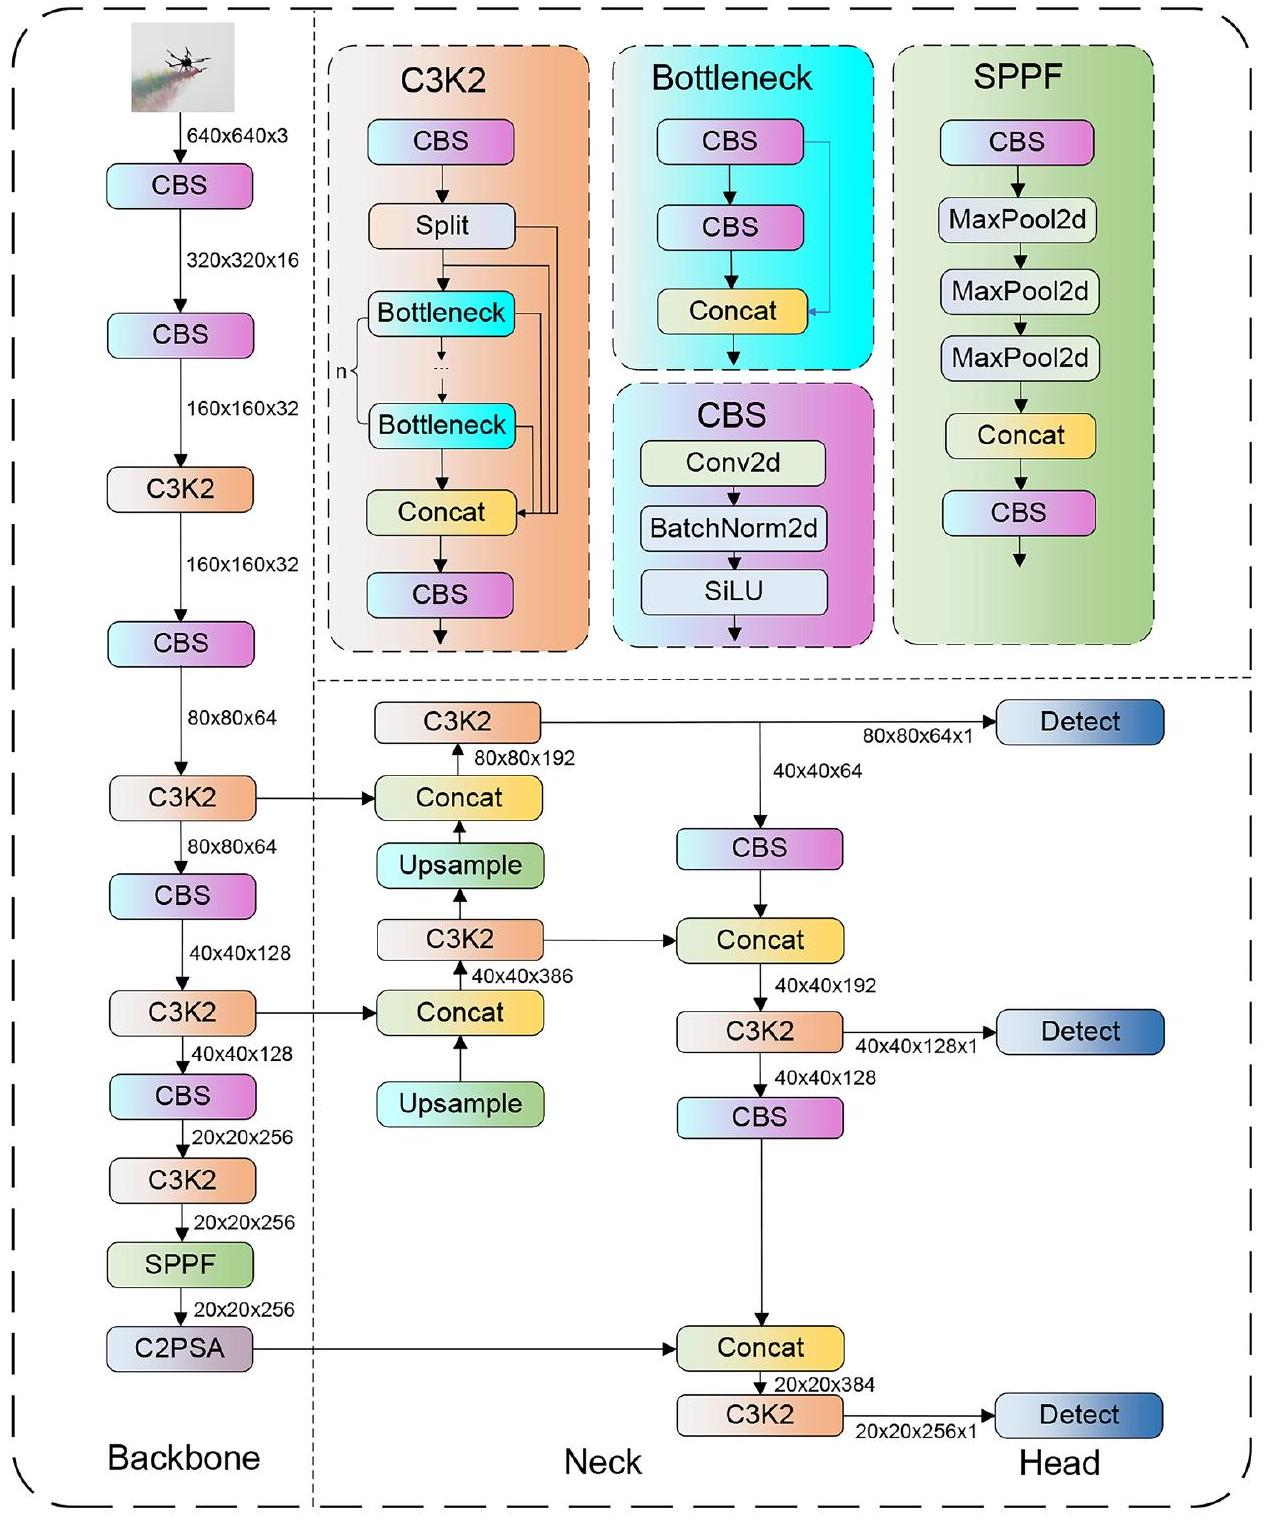
\includegraphics[max width=\textwidth, center]{2025_08_05_34f8389150f57116e76bg-04}

Fig. 1. The structure of YOLO11.\\
modeling. This design achieves efficient inference while maintaining an optimal balance between speed and accuracy.


\begin{align*}
& \operatorname{Re} L U 6(x)=\min (\max (0, x), 6)  \tag{1}\\
& H-\operatorname{swish}(x)=x \frac{\operatorname{Re} L U 6(x+3)}{6} \tag{2}
\end{align*}


As illustrated in Fig. 3, the LCbackbone module begins by leveraging depthwise separable convolutions to break down convolution operations into two steps: first, depthwise convolutions independently extract spatial features from each channel; second, pointwise convolutions using a $1 \times 1$ kernel enable cross-channel feature fusion. To further optimize performance, the module employs the H -Swish activation function, as defined in Eqs. (1) and (2), which replaces complex exponential operations with a combination of a hard sigmoid and linear transformations, improving computational efficiency. An SE module is integrated at the end of the network to capture global information for each channel through global average pooling. The SE module generates adaptive channel weights via activation functions and fully connected layers, enhancing feature reweighting and representation. Additionally, a $5 \times 5$ convolutional kernel is incorporated in the deeper layers of the network to expand the receptive field, enabling the capture of broader contextual information. Finally, a $1 \times 1$ convolutional layer with 1280 dimensions is added after the global average pooling layer to strengthen the model's global feature fitting capability.\\
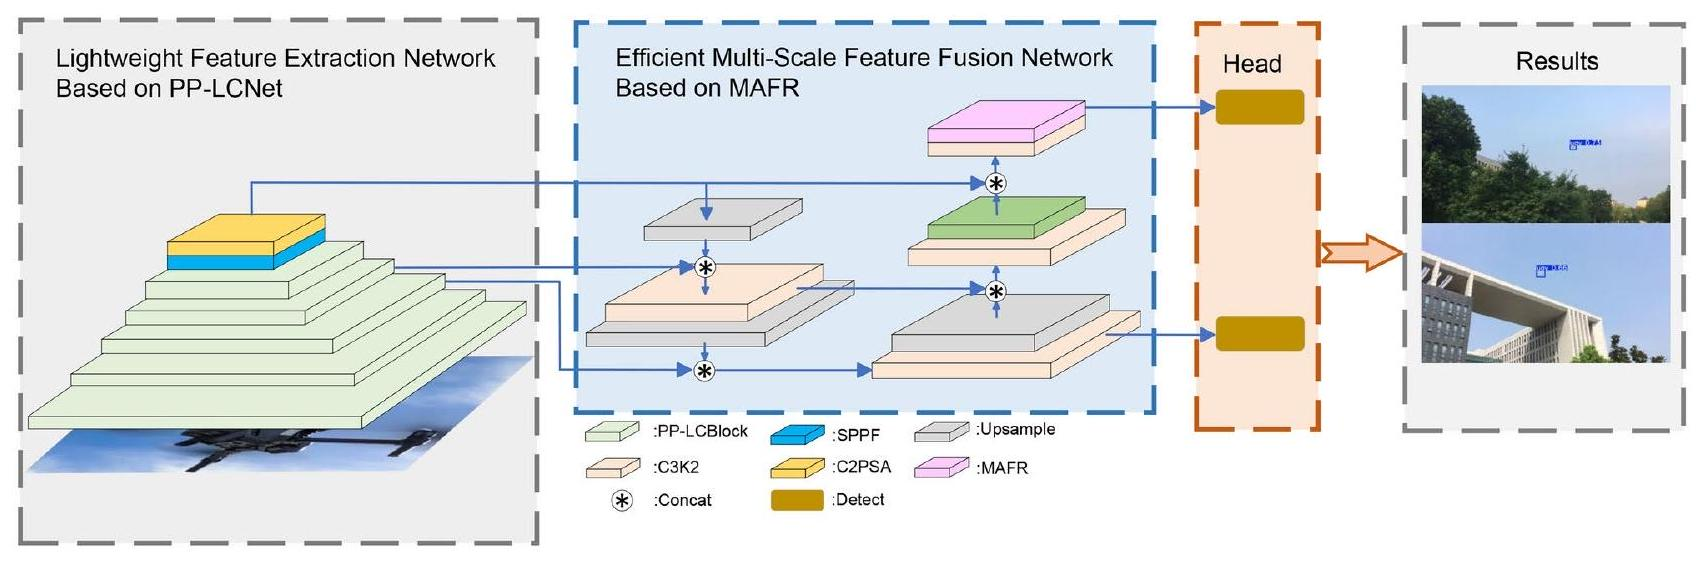
\includegraphics[max width=\textwidth, center]{2025_08_05_34f8389150f57116e76bg-05(1)}

Improved YOLO Network Structure\\
Fig. 2. Optimization techniques in LMWP-YOLO include the development of a novel feature extraction network utilizing PP-LCNet as a replacement for the original backbone. Furthermore, the multidimensional collaborative attention incorporates the multi-scale feature fusion module to create an enhanced feature fusion network, which replaces the original neck layer.\\
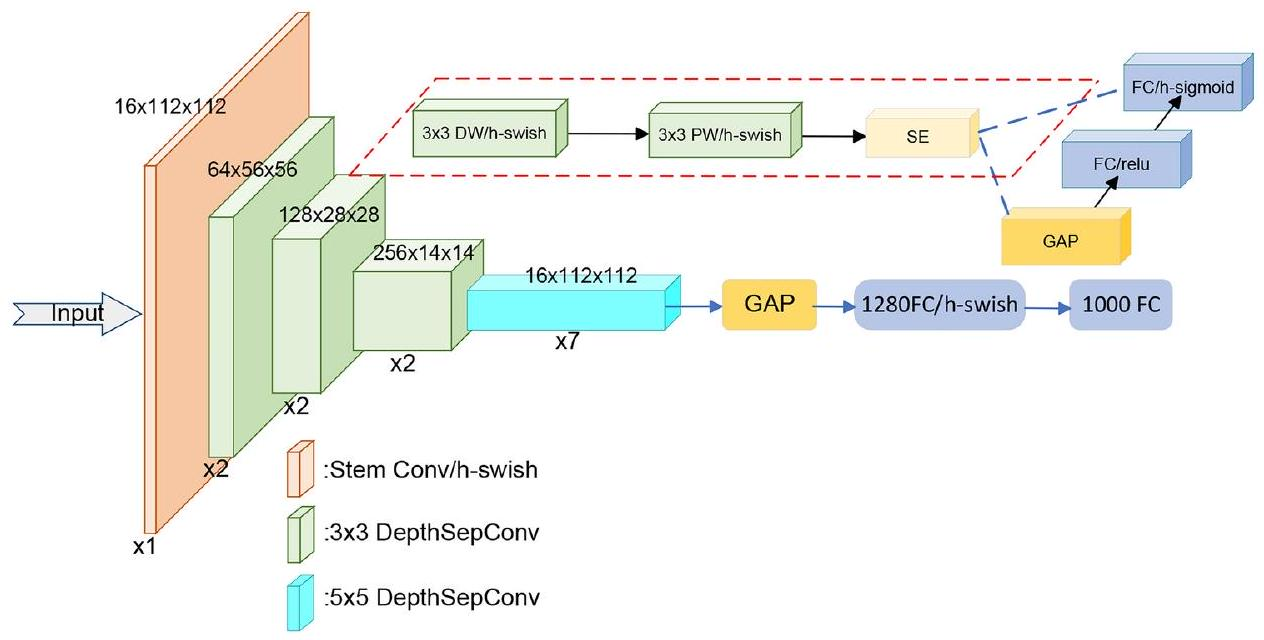
\includegraphics[max width=\textwidth, center]{2025_08_05_34f8389150f57116e76bg-05}

Fig. 3. Improvement scheme at the backbone combined with the PP-LCNet.

\section*{The improved neck incorporates a multidimensional collaborative attention mechanism alongside multi-scale fusion and residual connections to enhance performance}
In small object detection tasks for drones, small objects occupy minimal space in feature maps, leading to poor feature representation. In YOLO11, the neck layer's convolutions and C3K2 module enhance perception through multi-scale fusion, but small object features are often lost or diluted. To address this, we propose the MAFRneck layer, incorporating multidimensional collaborative attention ${ }^{41}$ to capture relationships between features. A lightweight multi-scale fusion module, combined with the SE module and residual connections ${ }^{42}$, optimizes feature extraction. Micro residual blocks improve gradient propagation, and adjustments to the neck layer enhance high-resolution feature representation.

As shown in Fig. 4, MAFR models the collaborative relationships among the channel, width, and height dimensions of input features by capturing attention weights for each dimension. It processes a feature tensor $F \in R^{C \times H \times W}$, using global average and standard deviation pooling to extract statistical features along the channel dimension, as described in Eqs. (3) and (4).


\begin{equation*}
z_{c}^{a v g}=\frac{1}{H \times W} \sum_{i=1}^{H} \sum_{j=1}^{W} F_{c, i, j} \tag{3}
\end{equation*}


\begin{center}
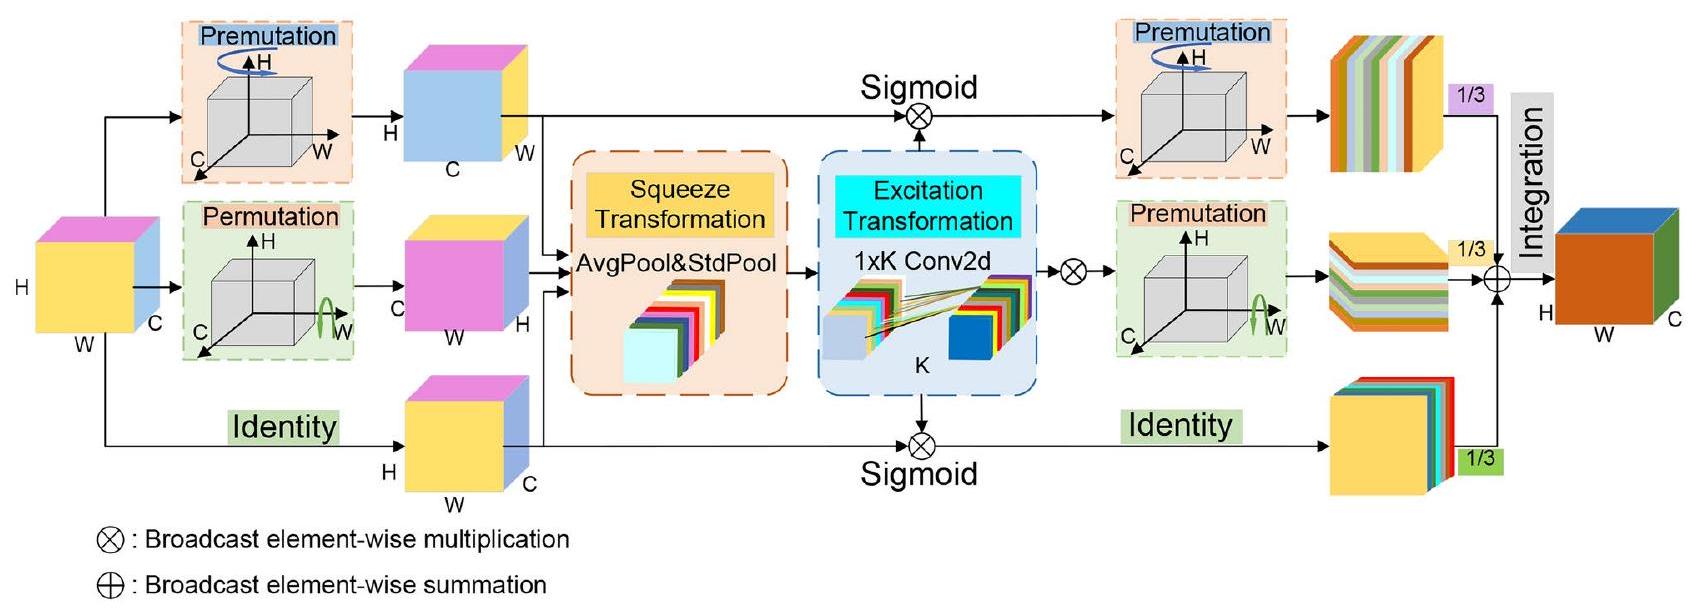
\includegraphics[max width=\textwidth]{2025_08_05_34f8389150f57116e76bg-06}
\end{center}

Fig. 4. Enhanced contextual information capture.


\begin{equation*}
z_{c}^{s t d}=\sqrt{\frac{1}{H \times W} \sum_{i=1}^{H} \sum_{j=1}^{W}\left(F_{c, i, j}-z_{c}^{a v g}\right)^{2}} \tag{4}
\end{equation*}


After concatenating the mean and standard deviation, channel attention weights are generated through a fully connected layer, as shown in Eq. (5).


\begin{equation*}
S_{C}=\sigma\left(W_{2} \delta\left(W_{1}\left[z_{c}^{a v g}, z_{c}^{s t d}\right]\right)\right) \tag{5}
\end{equation*}


Here, $W_{1}$ and $W_{2}$ are learnable weights, $\delta$ represents the ReLU activation function, $\sigma$ denotes the Sigmoid activation function, and [, ] indicates concatenation. The feature map is aggregated along the width dimension to produce descriptors for the height dimension, with a similar process used to generate height attention weights.


\begin{equation*}
z_{h}=\frac{1}{W} \sum_{j=1}^{W} F_{:, h, j} \tag{6}
\end{equation*}


Similarly, the feature map is globally aggregated along the height dimension to generate feature descriptors for the width dimension.


\begin{equation*}
z_{w}=\frac{1}{H} \sum_{i=1}^{H} F_{:, i, w} \tag{7}
\end{equation*}


The attention weights from the three dimensions are then individually applied to the input features.


\begin{equation*}
F_{C}^{\prime}=F \odot S_{C}, F_{H}^{\prime}=F \odot S_{H}, F_{W}^{\prime}=F \odot S_{W} \tag{8}
\end{equation*}


Here, $\odot$ represents element-wise multiplication. The three calibrated feature sets are then fused to generate multidimensional calibrated features.


\begin{equation*}
F^{\prime}=\frac{1}{3}\left(F_{C}^{\prime}+F_{H}^{\prime}+F_{W}^{\prime}\right) \tag{9}
\end{equation*}


Multi-scale features are crucial for small object detection. To address this, as illustrated in Fig. 5, a lightweight multi-scale fusion module uses grouped convolutions for feature extraction and $1 \times 1$ convolutions for integration, reducing parameter complexity. An SE module captures inter-channel relationships, while residual connections improve feature retention and gradient propagation. A micro residual block is added after the multi-scale fusion module to enhance feature extraction. It uses two $3 \times 3$ convolutions and batch normalization to extract finegrained features, with residual connections preserving original information and detailed small object features.

Traditional neck layers like FPN and PANet rely on P4 and P5 layers to capture large object features, limiting small object detection. To address this limitation, this study modifies the neck structure by decreasing the P4 and P5 layers and introducing a P2 layer, designed for small object features. The P2 layer processes higher-resolution feature maps, enhancing small object detail capture while reducing computational complexity. The full MAFRNeck structure is shown in Fig. 6.\\
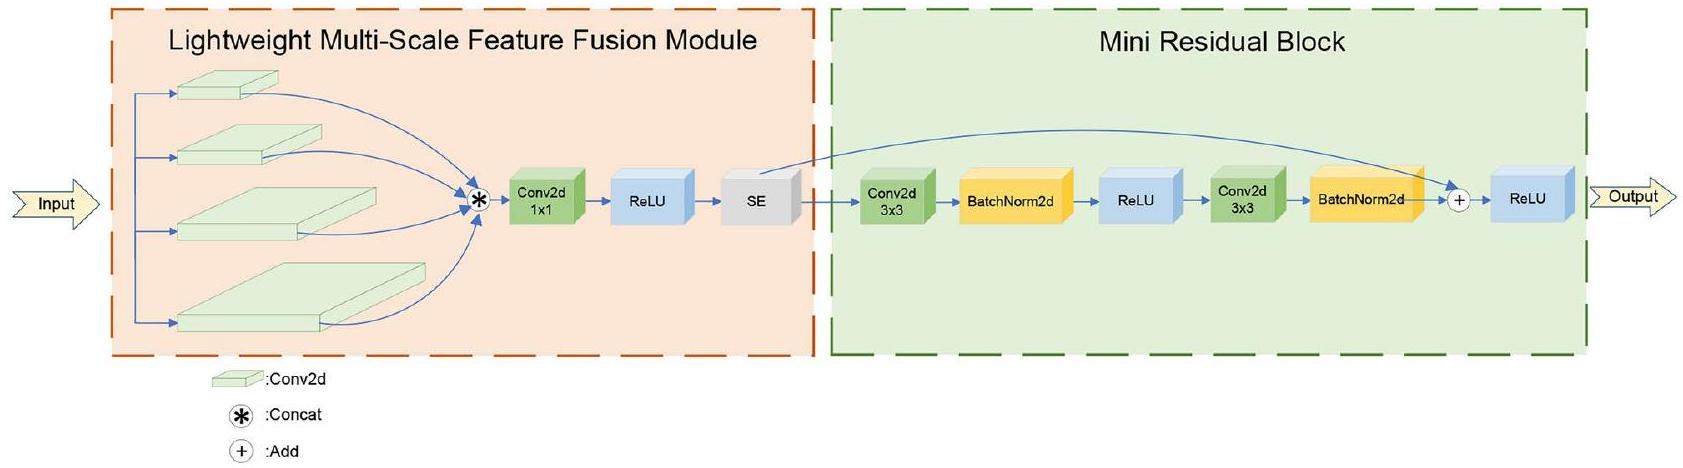
\includegraphics[max width=\textwidth, center]{2025_08_05_34f8389150f57116e76bg-07(1)}

Fig. 5. Multi-scale feature fusion and residual connect module.\\
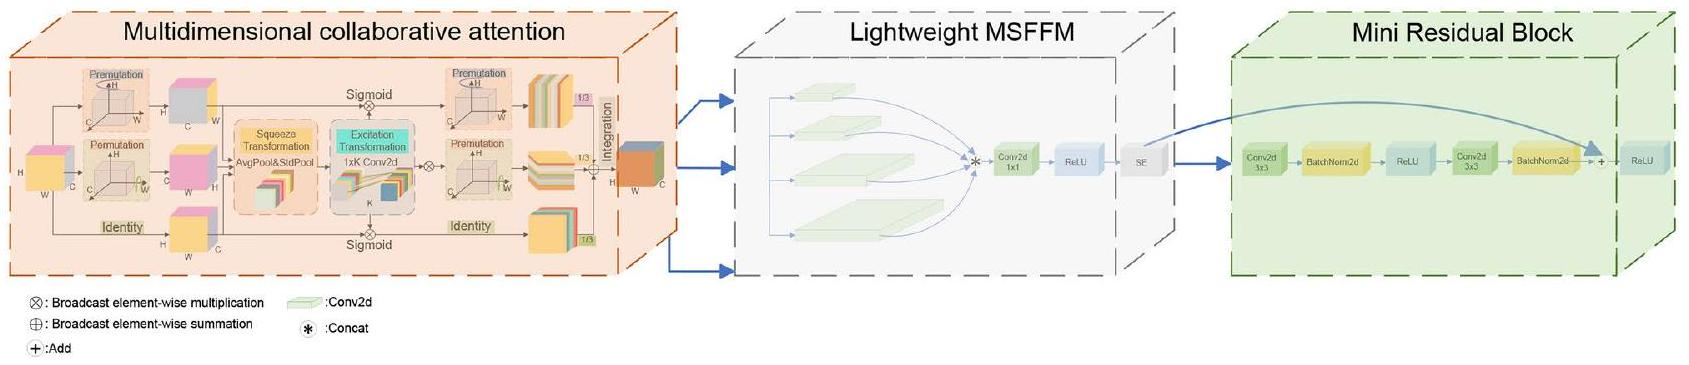
\includegraphics[max width=\textwidth, center]{2025_08_05_34f8389150f57116e76bg-07}

Fig. 6. The structure of improved MAFR network.

\section*{Improved loss function based on area-weighted Wasserstein loss}
In drone small object detection tasks, challenges arise due to the small size of targets, complex backgrounds, and dense distributions. Consequently, the robustness and accuracy of bounding box similarity measures are crucial for detection performance. However, YOLO11's loss function, which relies on an IoU-based bounding box regression mechanism, has notable limitations. It is highly sensitive to small positional shifts in targets and encounters gradient vanishing issues when bounding boxes have no overlap or are fully enclosed. To overcome these limitations, this study introduces a novel loss function. The key idea is to model the similarity between bounding boxes as a two-dimensional Gaussian distribution ${ }^{43}$ and use the Wasserstein distance to compute the distributional difference between predicted and ground-truth boxes. A dynamic weighting mechanism based on target area prioritizes the optimization of small objects, while the inclusion of a scale difference term improves the loss function's adaptability to multi-scale scenarios.

The horizontal bounding box $R=\left(c_{x}, c_{y}, w, h\right)$ is represented as a two-dimensional Gaussian distribution. In this representation, ( $c_{x}, c_{y}$ ) denotes the center point coordinates, while w and h indicate the width and height of the box, respectively. The Gaussian distribution corresponding to this representation is defined as:


\begin{equation*}
N(x \mid \mu, \Sigma)=\frac{1}{2 \pi|\Sigma|^{1 / 2}} \exp \left(-\frac{1}{2}(x-\mu)^{T} \Sigma^{-1}(x-\mu)\right) \tag{10}
\end{equation*}


Here, $\mu=\left[\begin{array}{l}c_{x} \\ c_{y}\end{array}\right], \Sigma=\left[\begin{array}{cc}\frac{w^{2}}{4} & 0 \\ 0 & \frac{h^{2}}{4}\end{array}\right] . \mu$ represents the center of the Gaussian distribution, corresponding to the center point of the bounding box. $\Sigma$ is the covariance matrix, which defines the width and height of the box. Using this model concept, the predicted bounding box A and the ground truth bounding box B can be represented as $N_{A}\left(\mu_{A}, \Sigma_{A}\right)$ and $N_{B}\left(\mu_{B}, \Sigma_{B}\right)$, respectively. The 2D Wasserstein distance is defined as:


\begin{equation*}
W_{2}^{2}\left(N_{A}, N_{B}\right)=\left\|\mu_{A}-\mu_{B}\right\|_{2}^{2}+\operatorname{Tr}\left(\Sigma_{A}+\Sigma_{B}-2\left(\Sigma_{B}^{1 / 2} \Sigma_{A} \Sigma_{B}^{1 / 2}\right)^{1 / 2}\right) \tag{11}
\end{equation*}


This can be simplified as:


\begin{equation*}
W_{2}^{2}\left(N_{A}, N_{B}\right)=\left\|\mu_{A}-\mu_{B}\right\|_{2}^{2}+\left\|\Sigma_{A}^{1 / 2}-\Sigma_{B}^{1 / 2}\right\|_{F}^{2} \tag{12}
\end{equation*}


Coupled with bounding boxes $R_{A}$ and $R_{B}$, the equation can be formulated as:


\begin{equation*}
W_{2}^{2}\left(N_{A}, N_{B}\right)=\left\|\left[c x_{A}, c y_{A}, \frac{w_{A}}{2}, \frac{h_{A}}{2}\right]^{T},\left[c x_{B}, c y_{B}, \frac{w_{B}}{2}, \frac{h_{B}}{2}\right]^{T}\right\|_{2}^{2} \tag{13}
\end{equation*}


To constrain the 2D Wasserstein distance within the range $(0,1)$, the typical 2D Wasserstein distance can be expressed as:


\begin{equation*}
N W D\left(N_{A}, N_{B}\right)=\exp \left(-\frac{\sqrt{W_{2}^{2}\left(N_{A}, N_{B}\right)}}{C}\right) \tag{14}
\end{equation*}


C is the normalization constant, determined based on the statistical information of the dataset. The schematic diagram of the predicted box and ground truth box is shown in Fig. 7. The box loss function can be expressed as:


\begin{equation*}
L_{b o x}=1-N W D\left(N_{A}, N_{B}\right) \tag{15}
\end{equation*}


The classification loss function can be expressed as:


\begin{equation*}
L_{c l s}=\sum_{i=0}^{s^{2}} \sum_{j=0}^{B} 1_{i j}^{o b j} \sum_{c \in N_{C}}\left[\hat{p}_{i}(c) \log \left(p_{i}(c)\right)+(1-\hat{p}) \times \log \left(1-p_{i}(c)\right)\right] \tag{16}
\end{equation*}


In this context, $S^{2}$ represents the total number of grid cells in the image, B denotes the number of bounding boxes, $N_{C}$ refers to the number of object categories, and $p_{i}$ represents the confidence score of bounding box i for class C . The object confidence loss function is defined as:


\begin{equation*}
L_{o b j}=\sum_{i=0}^{s^{2}} \sum_{j=0}^{B}\left[1_{i j}^{o b j}\left(C_{i}-\hat{C}_{i}\right)-1_{i j}^{n o o b j}\left(C_{i}-\hat{C}_{i}\right)\right] \tag{17}
\end{equation*}


Here, $1_{i j}^{o b j}$ represents the object located in cell i , selected by the j -th bounding box. $C_{i}$ and $\hat{C}_{i}$ denote the predicted and actual confidence levels, respectively. The loss function for iterative computation is defined as the sum of the three previously described functions, formulated as:


\begin{equation*}
L=\lambda_{b o x} \cdot L_{b o x}+\lambda_{c l s} \cdot L_{c l s}+\lambda_{o b j} \cdot L_{o b j} \tag{18}
\end{equation*}


In this case, $\lambda_{b o x}, \lambda_{c l s}$, and $\lambda_{o b j}$ denote the respective weights assigned to each loss function. In the approach described, the bounding box is modeled as a two-dimensional Gaussian distribution. The normalized Wasserstein distance is employed to precisely quantify differences in the position and size of the bounding boxes, ensuring smooth gradient calculations even in scenarios without overlap or containment relationships.

This paper subsequently introduces a dynamic weighting mechanism based on target area. A sigmoid mapping is applied to the target area, allowing the optimization weights for bounding box regression to be dynamically adjusted according to target size. Smaller targets are assigned higher weights, increasing their priority during optimization and significantly enhancing the model's sensitivity to detecting small objects. Finally, a relative scale difference term is added to the loss function to explicitly quantify the width and height differences between predicted and ground truth boxes. This encourages more precise predictions of target dimensions, thereby improving detection performance across multi-scale scenarios.

\section*{Pruning method for the drone detection network}
Efficiently extracting and utilizing small object features under limited computational resources is a critical challenge in drone-based small object detection tasks. YOLO11 improves feature extraction and object perception through multi-scale feature fusion in the backbone's convolutional layers and the neck layer. However, many unpruned filters in the convolutional layers introduce redundancy, as small object features occupy only a tiny portion of the convolutional feature maps. This results in weak feature activation for some filters, rendering them ineffective and wasting computational resources. To address this issue, this paper introduces a pruning-based\\

Fig. 7. The scheme of area-weighted Wasserstein loss function.\\
optimization strategy into the YOLO11 network structure ${ }^{44}$. The strategy involves evaluating the importance of each filter in the convolutional neural network and removing redundant filters, along with their associated feature maps, that contribute minimally to the network's output. This approach reduces both computational cost and the number of network parameters, enhancing the model's efficiency.

Specifically, the importance of each filter in a convolutional layer is evaluated using the L1-norm. For the j-th filter Fi in the i-th layer, represented by the weight tensor $F_{i, j} \in R^{n_{i} \times k \times k}$, the L1-norm is defined as:


\begin{equation*}
\left\|F_{i, j}\right\|_{1}=\sum_{l=1}^{n_{i}} \sum_{m=1}^{k} \sum_{n=1}^{k}\left|K_{l, m, n}\right| \tag{19}
\end{equation*}


Here, $n_{i}$ represents the number of input channels, $\mathrm{k} \times \mathrm{k}$ denotes the kernel size, and $K_{l, m, n}$ indicates the weight value of the $j$-th filter in the i-th layer at channel 1 and position ( $m, n$ ). Filters in each convolutional layer are ranked by their L1-norm, and those with the lowest values are selected for removal. As shown in Fig. 8, the pruned filters correspond to feature maps that are also removed, subsequently affecting the convolutional kernels in the following layers.

\section*{Experimental results and analysis}
This section evaluates the proposed model's detection performance on datasets and compares it with current object detection algorithms to demonstrate its superiority.

\section*{Dataset and training}
With the increasing adoption of civilian drones, their applications in daily life are expanding rapidly. Publicly available datasets offer a variety of drone images captured under diverse environmental conditions. However, many of these datasets lack sufficient small-object feature information, which can compromise the accuracy of models in detecting small drone targets. To address this limitation, this study utilizes the publicly available TIBNet small drone target dataset ${ }^{45}$, which consists of a total of 2850 images of various types of drones, including multi-rotor and fixed-wing drones, with an approximate distance of 500 m . The dataset covers scenes ranging from daytime to nighttime under various lighting conditions. In this study, 2565 images are selected as the training set, and 285 images are used as the validation set. The dataset annotates small drone targets using text files containing five columns: class label, center coordinates of the bounding box ( x and y ), width, and height. Figure 9 presents the data distribution of drone classes and the bounding box specifications within the training set. To ensure consistency in controlled experiments, all models use the same hyperparameters, with an input image size fixed at $640 \times 640$. The model was trained for 100 epochs on 2565 images from the training set using an A100, with a batch size of 48 and the AdamW optimizer.

The experimental environment in this paper is based on the Ubuntu 20.04 operating system, with an Tensor Core A100 GPU, 40GB of memory. The programming language used is Python 3.9.11, and the deep learning model is built using PyTorch 1.10.0, cudnn 8.2.0, and torchvision 0.12.0. The computational library used is numpy 1.23.3, and parallel computing is supported by the NVIDIA CUDA Toolkit 11.3.0. The code is available at \href{https://github.com/Surprise-Zhou/LMWP-YOLO}{https://github.com/Surprise-Zhou/LMWP-YOLO}.

\section*{Accuracy evaluation}
Drone small object detection models are evaluated using four metrics: precision $(\mathrm{P})$, recall $(\mathrm{R})$, F1-score, and mean average precision (mAP), with their calculation formulas provided.


\begin{equation*}
P=\frac{T P}{T P+F P} \tag{20}
\end{equation*}


\begin{center}
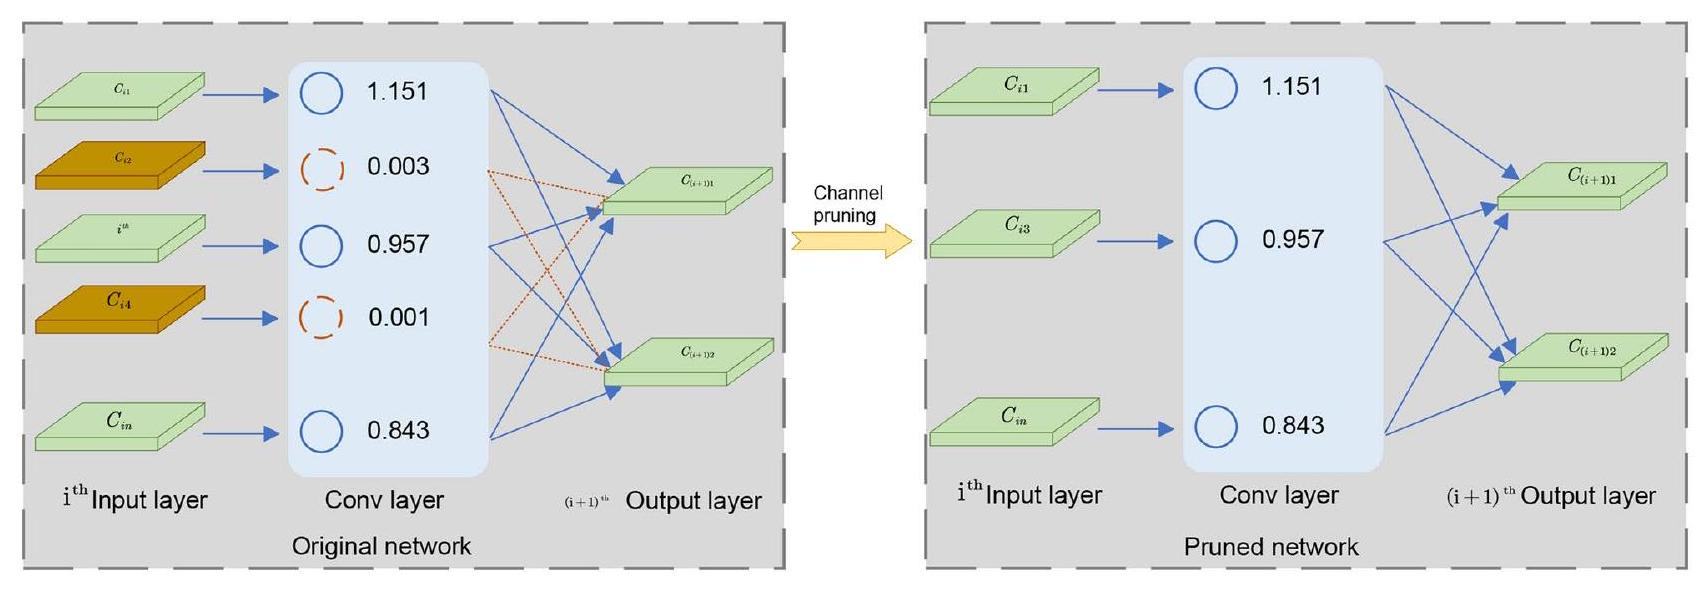
\includegraphics[max width=\textwidth]{2025_08_05_34f8389150f57116e76bg-09}
\end{center}

Fig. 8. Schematic diagram of channel pruning method.\\
study introduces LMWP-YOLO, a lightweight object detection model specifically designed for detecting small, multi-scale, and low-latency drone targets over long distances.

This study enhances YOLO11n's backbone network by integrating the LCbackbone architecture, which employs depthwise separable convolutions and the H-Swish activation function. These improvements optimize computational efficiency and feature extraction, enabling the model to perform effectively on resourceconstrained devices. Furthermore, a novel MAFR module is introduced in the neck layer. This module incorporates a multidimensional collaborative attention mechanism to strengthen feature dependencies across dimensions and efficiently extract multi-scale features. Additionally, the SE module and residual connections refine feature representation and enhance gradient propagation. The loss function is also improved by incorporating the normalized Wasserstein distance, which mitigates IoU's sensitivity to positional and shape deviations in small targets. Finally, a pruning strategy is implemented to eliminate low-importance network channels and convolutional kernels, effectively reducing model redundancy.

This study introduces the one-stage LMWP-YOLO model and evaluates its performance against the baseline YOLO11n model. The results demonstrate that LMWP-YOLO achieves a lightweight design, enhances detection efficiency, and significantly improves recognition capabilities for small drone targets. This advancement offers an innovative and effective solution for the detection of small drone targets.

However, this study has several limitations. First, the dataset used does not include complex weather conditions such as strong winds, heavy fog, and snow, leaving the model's performance in adverse environments unverified. Second, although a multi-scale feature fusion module was introduced to enhance the feature representation of small targets, in high-density scenarios of small drone target detection, issues such as target occlusion and feature blurring may lead to missed detections. Lastly, while the loss function improves the robustness of target detection through a dynamic weighting mechanism, in scenarios involving small target swarms, the loss signal may be weakened due to the high-density target distribution, thereby affecting the model's accuracy in detecting small targets.

Future research should expand the dataset to include complex extreme weather conditions and diverse scenarios, thereby improving the model's generalization ability across various environments. Additionally, specialized detection modules for high-density drone swarms should be developed. For example, incorporating Transformer-based global feature modeling can enhance the model's capacity to capture complex relationships among multiple targets. In high-density target scenarios, dynamic multi-target distribution modeling mechanisms can be employed to group and separate swarm features, effectively mitigating the impact of occlusion on detection outcomes. Moreover, designing a jointly optimized loss function for extreme weather and swarm scenarios would enable dynamic adjustment of loss weights across targets, thereby improving the precision of single-target detection within dense swarms. These advancements will further enhance the model's adaptability to extreme environments, offering a more comprehensive and robust solution for detecting small drone swarms.

To address this, we designed a new C3TR module, based on a Transformer encoder ${ }^{47}$, following the MAFR in the neck layer to validate the effectiveness of global feature modeling by Transformers. As shown in Fig. 16, this module uses a self-attention mechanism to capture long-range dependencies in the image, overcoming the limitations of the C3K2 module in modeling such dependencies. Additionally, it explicitly captures the contextual information of occluded targets, helping to accurately distinguish these targets and reduce the likelihood of missed detections due to occlusion.

Additionally, we introduce an occlusion-aware factor in the loss function, which estimates local density by calculating the Intersection over Union (IoU) between predicted boxes, enabling effective detection of drone swarms. We also incorporate illumination invariance adjustments through simple brightness consistency constraints to enhance the model's robustness. Finally, we add a relative scale difference term to the loss function to explicitly measure the relative width and height differences between predicted and ground truth boxes. This term, combined with dynamic weights, the occlusion factor, and temperature coefficients, optimizes the stability and adaptability of the loss function.\\
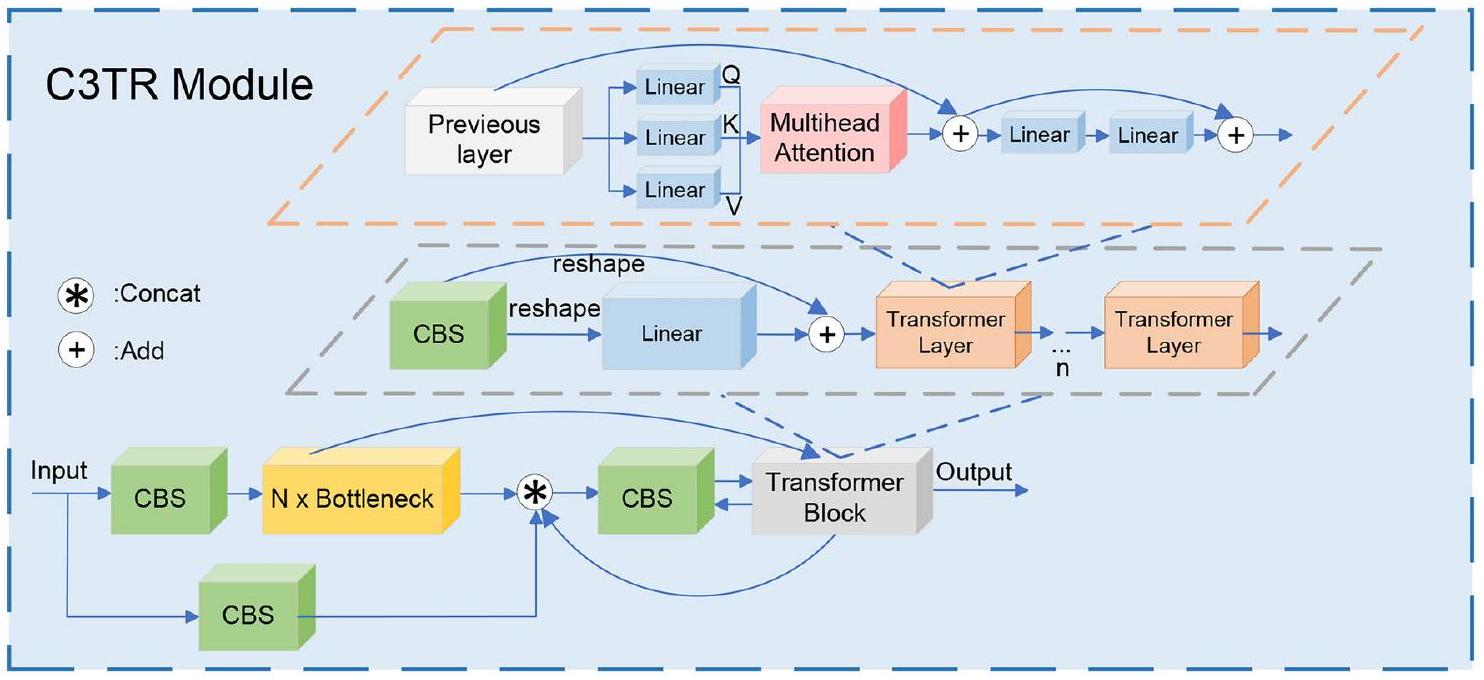
\includegraphics[max width=\textwidth, center]{2025_08_05_34f8389150f57116e76bg-17}

Fig. 16. The structure of C3TR module.

\begin{center}
\begin{tabular}{|l|l|l|l|l|l|l|l|l|}
\hline
Methods & LCbackbone & MAFR & AWLoss & C3TR & mAP@0.5 (\%) & mAP@0.95 (\%) & Parameters (M) & Model size (MB) \\
\hline
YOLO11n &  &  &  &  & 94.0 & 52.6 & 2.59 & 5.20 \\
\hline
Methods & $\checkmark$ & $\checkmark$ & $\checkmark$ & $\checkmark$ & 97.1 & 62.6 & 1.52 & 3.3 \\
\hline
\end{tabular}
\end{center}

Table 4. Results of comparative experiments on the UAVSwarm dataset.

To evaluate the detection performance of our innovative designs "LCbackbone," "MAFR," "AWLoss," and "C3TR" in drone swarm detection, we conducted comparison experiments with the baseline model using the drone swarm dataset. The drone swarm dataset is derived from the publicly available UAVSwarm dataset ${ }^{48}$. These experiments assessed the impact of the algorithmic improvements, focusing primarily on the global information modeling capability of the C3TR module. The evaluation metrics include mean average precision ( mAP ) and model parameters. The results on the drone swarm dataset are presented in Table 4.

The results in Table 4 show that our method outperforms the baseline model in key performance metrics, with mAP@0.5 and mAP@0.95 increasing by $3.3 \%$ and $19.0 \%$, respectively. These improvements are largely attributed to the newly designed C3TR module in the neck layer. The module effectively captures global contextual information through the self-attention mechanism of the Transformer. This enables the model to better understand the relationships between different regions, particularly in the context of drone swarm detection, where multiple dispersed swarm individuals are involved, and enhances the modeling of long-range dependencies.

\section*{Conclusion}
This study presents LMWP-YOLO, an enhanced lightweight detection framework for long-distance small drone target detection. The framework integrates lightweight network components, multi-scale feature fusion modules, and dynamically optimized loss functions.

\section*{References}
\begin{enumerate}
   \item **[39] Cui et al.**: This paper introduces PP-LCNet, a lightweight convolutional neural network optimized for CPU efficiency using depthwise separable convolutions, efficient activations like H-Swish, and Squeeze-and-Excitation modules to balance speed and accuracy in image classification tasks. (https://doi.org/10.48550/arXiv.2109.15099)
   \item **[40] Hu et al.**: This paper presents Squeeze-and-Excitation (SE) networks, which improve convolutional neural network performance by modeling inter-channel dependencies through global average pooling and adaptive recalibration to emphasize informative features. (https://doi.org/10.1109/CVPR.2018.00745)
   \item **[41] Yu et al.**: This work proposes Multidimensional Collaborative Attention (MCA), a mechanism that captures collaborative relationships across channel, height, and width dimensions in deep convolutional networks to enhance image recognition by adaptively weighting features based on global pooling and fully connected layers. (https://doi.org/10.1016/j.engappai.2023.107079)
   \item **[42] He et al.**: This study develops deep residual learning (ResNet), a framework that uses skip connections to enable training of very deep neural networks by alleviating vanishing gradients and improving feature propagation for image recognition. (https://doi.org/10.1109/CVPR.2016.90)
   \item **[43] Wang et al.**: This paper introduces Normalized Gaussian Wasserstein Distance (NWD) for tiny object detection, modeling bounding boxes as Gaussian distributions to compute robust similarity measures that address limitations of traditional IoU in small-target scenarios. (https://doi.org/10.48550/arXiv.2110.13389)
   \item **[44] Li et al.**: This work proposes a pruning method for efficient ConvNets that ranks and removes low-importance filters using L1-norm to reduce model size and computational cost while preserving accuracy in deep networks. (https://doi.org/10.48550/arXiv.1608.08710)
   \item **[47] Dosovitskiy et al.**: This paper presents Vision Transformers (ViT), an architecture that applies transformer encoders to image patches treated as sequences, enabling scalable image recognition through self-attention for capturing long-range dependencies. (https://doi.org/10.48550/arXiv.2010.11929)
\end{enumerate}

\end{document}